\documentclass[10pt,a4paper]{article}
\usepackage[T1]{fontenc}
\usepackage[scaled]{helvet}
\usepackage{cite}
\usepackage{url}
\usepackage{graphicx}
\usepackage{listings}
\usepackage{float}
\usepackage{amsmath}
\usepackage{listings}
\usepackage{color}
 
\definecolor{dkgreen}{rgb}{0,0.6,0}
\definecolor{gray}{rgb}{0.5,0.5,0.5}
\definecolor{mauve}{rgb}{0.58,0,0.82}
\lstset{ %
  language=Octave,                % the language of the code
  basicstyle=\footnotesize,           % the size of the fonts that are used for the code
  numbers=left,                   % where to put the line-numbers
  numberstyle=\tiny\color{gray},  % the style that is used for the line-numbers
  stepnumber=1,                   % the step between two line-numbers. If it's 1, each line 
                                  % will be numbered
  numbersep=5pt,                  % how far the line-numbers are from the code
  backgroundcolor=\color{white},      % choose the background color. You must add \usepackage{color}
  showspaces=false,               % show spaces adding particular underscores
  showstringspaces=true,         % underline spaces within strings
  showtabs=false,                 % show tabs within strings adding particular underscores
  frame=none,                   % adds a frame around the code
  rulecolor=\color{black},        % if not set, the frame-color may be changed on line-breaks within not-black text (e.g. commens (green here))
  tabsize=4,                      % sets default tabsize to 2 spaces
  breaklines=true,                % sets automatic line breaking
  breakatwhitespace=false,        % sets if automatic breaks should only happen at whitespace
  keywordstyle=\color{blue},          % keyword style
  commentstyle=\color{dkgreen},       % comment style
  stringstyle=\color{mauve},         % string literal style
  escapeinside={\%*}{*)},            % if you want to add LaTeX within your code
  morekeywords={*,...}               % if you want to add more keywords to the set
}
\usepackage{amssymb}
\usepackage{fancyhdr}
\usepackage{lastpage}
\floatstyle{boxed} 
\restylefloat{figure}
\renewcommand*\familydefault{\sfdefault}
\title{Hash Tables}
\author{David Lynch - david.lynch@raglansoftware.com }
\begin{document}
\maketitle
\begin{abstract}
A hash table is an interesting data structure for a number of reasons. Firstly, you'll see them anywhere you might want to maintain a keyed list of anything, as the $O(1)$ nature of the retrieval is very desirable the for applications that refer to keyed list by the key value itself. More interestingly, due to space constraints the this performance may not remain constant for the duration of the existence of the hash table. This makes for a simple example of a data structure that requires work to maintain its key property. 
\end{abstract}
\section{Background}
Many applications require a dynamic that supports only the operations {\it INSERT, SEARCH} and {\it DELETE}. A hash table is an effective data structure for implementing dictionaries. Searching for an element in a hash has an upper bound of \Theta$(n)$ but given reasonable assumptions about the hash table, retrieval can be put at $O(n)$. A hash table generalizes the simpler notion of an array by using direct addressing as a means to implement an explicit key. When the number of keys store is small relative to the number of possible keys, hash tables are an effective alternative to maintaining an complimentary array of direct addresses. Conceptually, the array index is computed from the {\bf key} by applying a {\bf hash function} to the key. When {\bf collisions} occur in a hash table {\bf chaining} is used to resolve the key-pair mapping. 
\section{Direct Address Tables}
When the {\it universe} of possible keys is small, direct-address tables are useful. Each element has a key from the universe $U={0,1...,m-1}$ where $m$ is not too large by some measure and the hash function $h(k)$ enforces the rule that no two elements have the same key. Direct addressing implementation is relatively trivial. Figure \ref{diraddr} illustrates direct addressing. 
\end{figure}
\begin{figure}
\caption{Direct Address Tables \cite{INTROALG}}
\begin{center}
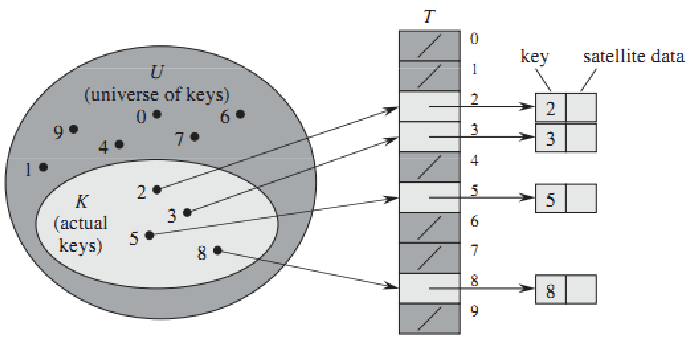
\includegraphics[scale=0.43]{../images/directaddtables.png}
\label{diraddr}
\end{center}
\end{figure}
\section{Hash Tables}
If $U$ is sufficiently large, storing a table $T$ of size $|U|$ may be impractical, or even impossible. Also, the set of keys $K$ that is actually stored may be so small relative to $U$ that most of the space allocated for $T$ would be wasted. For large $U$ therefore, direct address tables are not space efficient. When the set of keys $K$ stored in a dictionary is much smaller than the universe $U$ of all possible keys, a hash table, which manages key collisions is much more space efficient. In fact we can reduce the storage requirement to $O(|K|)$ while maintaining the $O(1)$ access time property on average. With direct addressing element with key $k$ is stored in slot $h(k)$ where $h$ key is a simple mapping. With hashing the function $h(k)$ is a hash function $H : U -> {0,1...m-1}$. Collisions in the hash space are minimized by clever design of H and and keeping $m << U$. Figure \ref{hashtable} shows this diagrammatically, and also shows how each slot degrades to a linked list in the presence of collisions. 
\begin{figure}
\caption{A hash table with chaining. \cite{INTROALG}}
\begin{center}
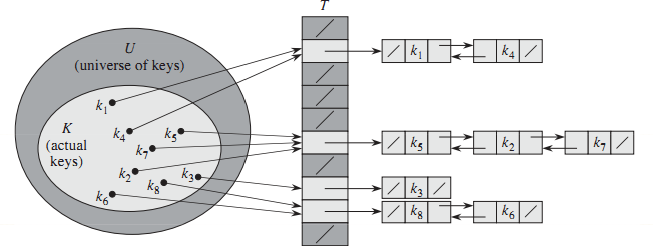
\includegraphics[scale=0.43]{../images/hashtable.png}
\label{hashtable}
\end{center}
\end{figure}
\section{Chaining}
Given a hash table $T$ with $m$ slots that stores $n$ elements {\bf load factor} for $T$, \Alpha as $n/m$ or the average number of elements stored in a chain. Retrieval performance degrades to that of a linked list, but insertion stays at constant time. The overall average-case performance of a hash table with chaining depends on how well the hash function distributes the set of keys to be stored among the $m$ available slots. If we assume that any given element is equally likely to hash to any of the $m$ slots, independently of where other elements have already hashed, then we assume {\bf simple, uniform hashing}. In a hash table in which collisions are resolved by chaining, an unsuccessful search and a successful search takes average case time $O(n+\Alpha}$
\section{Hash Functions}
A good hash function satisfies the simple uniform hashing assumption. It is very difficult to implement without {\it a priori} knowledge of the probability distribution of the drawing of keys. In practice we use hueristic techniques to create hash functions that perform well. In this case qualitative information about key distribution may be very useful. A good approach derives the hash value independently of any patterns that might exist in the data. Some applications of hash functions might require stronger properties than are provided by simple uniform hashing. We might get keys that are close to yield hash values that are far apart, or vice versa. Most hash functions assume the universe of keys to be the natural set of numbers N. If keys are not natural numbers we can find a way of interpreting them as such. 
\subsection{The Division Method}
A key $k$ is mapped to one of its $m$ slots by taking the remainder of $k$ divided by $m$ so that $h(k) = k mod (m)$. This can be performed in a single division and as such is quite fast. In this approach, the case where $m$ is a power of 2 needs to be avoided since the $p$ lower order bits of $k$

\\ FINISH AND RE_READ THIS \\

\section{Hash-Maps in Java}


\section{Further Reading}

http://tools.ietf.org/html/rfc1321 [MD5]
http://en.wikipedia.org/wiki/Bloom_filter [Bloom Filter]

\bibliography{../biblio/techfundamentals.bib}{}
\bibliographystyle{plain}
\begin{center}
{\small \copyright  David Lynch 2012. Do not reproduce without written permission.}
\end{center}
\end{document}
